\documentclass[11pt]{article}
\usepackage{enumerate}
\usepackage{amsmath}
\usepackage{blindtext}
\usepackage{multicol}
\usepackage{amsfonts}
\usepackage[left=1.5cm,top=2cm,right=1.5cm,bottom=2cm]{geometry}
\usepackage{graphicx}

\newcommand*\varhrulefill[1][0.4pt]{\leavevmode\leaders\hrule height#1\hfill\kern0pt}
\begin{document}

\begin{center}
    \textbf{MATEMÁTICA}
\end{center}

\noindent\varhrulefill[0.4mm]

\vspace{6pt}

\noindent \textbf{Notações}

\vspace{6pt}

$\mathbb{N}\quad = \{ 1,2,3, \dots \}$: o conjunto dos números naturais.

$\mathbb{R}\quad$: o conjunto dos números reais.

$\mathbb{C}\quad$: o conjunto dos números complexos.

$i \, \, \quad$: unidade imaginária, $i^2 = -1$.

\vspace{6pt}

\noindent Observação: Os sistemas de coordenadas considerados são os cartesianos retangulares.

\noindent\varhrulefill[0.4mm]

\vspace{6pt}

\parindent0em

\textbf{Questão 1.} Sejam  $A$,  $B$  e  $C$  conjuntos  contidos  num  mesmo  conjunto $U$. Seja $x$ um elemento de $U$, define-se: 
\[
C_B^A = \{ x \in U | x \in B \text{ e } x \not\in A \} 
\]
Então, $C_C^{(A \cup B)}$ é igual a:
\begin{multicols}{3}
    \begin{enumerate}[\bf A (\quad)]
        \item $C_C^A \cup C_C^B$
        \item $C_C^A \cap C_C^B$
        \item $C_A^B$
        \item O conjunto vazio
        \item n.d.a.
    \end{enumerate}
\end{multicols}

\textbf{Questão 2.} Sejam  $A$,  $B$  e  $D$  subconjuntos  não  vazios  o  conjunto  $\mathbb{R}$      dos      números      reais. Sejam as      funções $f: A \rightarrow B(y = f(x)) $ , $g: D \rightarrow B (x = g(t))$, e a função composta $g \circ f: E \rightarrow K$ (e,      portanto  $Z = (g \circ f)(t) = f(g(t))$.  Então  os  conjuntos  $E$  e  $K$  são tais que: 

\begin{multicols}{3}
\begin{enumerate}[\bf A (\quad)]
    \item $E \subset A$ e $K \subset D$
    \item $E \subset B$ e $K \supset A$
    \item $E \supset D$ e $D \neq E$ e $K \subset B$
    \item $E \subset D$ e $K \subset B$
    \item n.d.a.
\end{enumerate}
\end{multicols}


\textbf{Questão 3.} O volume de um tetraedro regular de aresta igual a $l$ é: 

\begin{multicols}{2}
    \begin{enumerate}[\bf A (\quad)]
        \item $l \sqrt{2}$
        \item $\dfrac{l^2 \sqrt{3}}{2}$
        \item $\dfrac{l^2 \sqrt{2}}{3}$
        \item $\dfrac{l^3 \sqrt{3}}{2}$
        \item n.d.a.
    \end{enumerate}
\end{multicols}

\textbf{Questão 4.} Seja $a > 0$ o $1^{\circ}$ termo de uma progressão aritmética de razão $r$ e também de uma progressão geométrica de razão $q = 2r \sqrt{3}/3a$.  A  relação  entre  $a$  e  $r$  para  que  o  terceiro  termo da progressão geométrica coincida com a soma dos 3 primeiros termos da progressão aritmética é: 

\begin{multicols}{5}
\begin{enumerate}[\bf A (\quad)]
    \item $r = 3a$
    \item $r = 2a$
    \item $r = a$
    \item $r =\sqrt{2a}$
    \item n.d.a.
\end{enumerate}
\end{multicols}

\textbf{Questão 5.} Sobre a raiz da equação podemos afirmar: 

\[
3^x - \frac{12}{3^{x-1}} + 3^{x-3} = \frac{23}{3^{x-2}}
\]

\begin{enumerate}[\bf A (\quad)]
    \item não é real
    \item é menor que -1
    \item está no intervalo $[0,6]$
    \item é um número primo
    \item n.d.a.
\end{enumerate}

\textbf{Questão 6.} A condição para que $\binom{n}{k}$ seja o dobro de $\binom{n}{k-1}$ é que:

\begin{multicols}{3}
    \begin{enumerate}[\bf A (\quad)]
        \item $n+1$ seja múltiplo de 3
        \item $n$ seja divisível por 3
        \item $n-1$ seja par
        \item $n=2k$
        \item n.d.a.
    \end{enumerate}
\end{multicols}

\textbf{Questão 7.} Sejam as matrizes

\[
A = 
\begin{bmatrix}
2 & 4\\
0 & 4
\end{bmatrix}, \,
B = 
\begin{bmatrix}
1 & 2\\
0 & 4
\end{bmatrix}, \,
Z =
\begin{bmatrix}
0 & 0\\
0 & 0
\end{bmatrix}, \,
I = 
\begin{bmatrix}
1 & 0\\
0 & 1
\end{bmatrix}
\]

Então temos:

\begin{multicols}{5}
\begin{enumerate}[\bf A (\quad)]
    \item $BA = I$
    \item $BA =AB$
    \item $A =2B$
    \item $AI = BZ$
    \item n.d.a.
\end{enumerate}
\end{multicols}

\textbf{Questão 8.} Seja a equação matricial

\[
\begin{bmatrix}
1 & 4 & 5 \\
3 &-1 & 7 \\
1 &-22&-11
\end{bmatrix}
\begin{bmatrix}
x \\
y \\
z
\end{bmatrix}
=
\begin{bmatrix}
0\\
0\\
0
\end{bmatrix}
\]

Podemos afirmar:

\begin{enumerate}[\bf A (\quad)]
    \item a equação tem uma e somente uma solução. 
    \item a equação tem duas e somente duas soluções. 
    \item a equação tem três e somente três soluções.
    \item a equação não tem solução.
    \item n.d.a.
\end{enumerate}

\textbf{Questão 9.} O    valor    da    expressão   $x = \dfrac{2 \tan \theta}{1 - \tan^2 \theta}$,    quando    $\cos \theta = -\dfrac{3}{7}$ e $\tan \theta < 0$, é:  

\begin{multicols}{3}
    \begin{enumerate}[\bf A (\quad)]
        \item $4\sqrt{10}/31$
        \item $-2\sqrt{10}/3$
        \item $2\sqrt{10}/15$
        \item $3\sqrt{10}/7$
        \item n.d.a.
    \end{enumerate}
\end{multicols}

\textbf{Questão 10.} $\left[ \dfrac{1 - \tan x}{1 + \tan x} \right]^2$ vale:

\begin{multicols}{3}
    \begin{enumerate}[\bf A (\quad)]
        \item $\dfrac{1 - 2\sin 2x}{1 + \sin 2x}$
        \item $\dfrac{1 + 2\sin 2x}{1 - \sin 2x}$
        \item $\dfrac{1 + \sin 2x}{1 + \sin 2x}$
        \item $\dfrac{1 - \sin 2x}{1 + \sin 2x}$
        \item n.d.a.
    \end{enumerate}
\end{multicols}

\newpage
\textbf{Questão 11.} Seja  $BC  =  CD$  no  quadrilátero  $ABCD$,  mostrado  na  figura abaixo. Então podemos garantir que: 

\begin{figure}[h]

\centering % para centralizarmos a figura
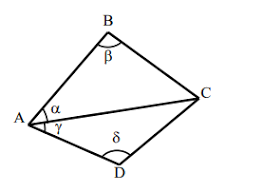
\includegraphics[width=7cm]{imgs/q11.png} % leia abaixo
\label{•}
\end{figure} 

\begin{enumerate}[\bf A (\quad)]
    \item $\dfrac{\sin \gamma}{\sin \delta} = \dfrac{\sin \alpha}{\sin \beta}$
    \item $\delta \alpha = \beta \gamma$
    \item $\tan \alpha \tan \beta = \tan \delta \tan \gamma$
    \item $BC^2 = AB. AB$
    \item n.d.a.
\end{enumerate}


\textbf{Questão 12.} A reta que passa pelas interseções das circunferências $x^2 + y^2 = 1$ e $(x - 1)^2 + (y - 1)^2 = 2$, é tal que:

\begin{enumerate}[\bf A (\quad)]
    \item  tem equação $\dfrac{3}{5}x - \dfrac{2}{3}y + \dfrac{1}{4} = 0$
    \item não passa pela origem.
    \item passa pela origem. 
    \item não é perpendicular à reta que passa pelos centros das circunferências.
    \item n.d.a.
\end{enumerate}


\textbf{Questão 13.} Os  zeros  da  função $P(x) = 3x^6 - 8x^5 + 3x^4 + 2x^3$:

\begin{enumerate}[\bf A (\quad)]
    \item todos inteiros.
    \item 2 imaginários puros e 4 reais
    \item todos racionais 
    \item 4 racionais e 2 irracionais
    \item n.d.a.
\end{enumerate}


\textbf{Questão 14.} A equação $x^n - 1$, onde $n$ é um número natural maior do que 5, tem:

\begin{enumerate}[\bf A (\quad)]
    \item 1  raiz  positiva,  1  raiz  negativa  e  $(n - 2)$  raízes  complexas quando $n$ é par. 
    \item 1 raiz positiva, $(n - 1)$ raízes não reais quando $n$ é par. 
    \item 1  raiz  negativa,  $(n - 1)$  raízes  complexas  quando  $n$  é  ímpar.
    \item 1  raiz  positiva,  1  raiz  negativa  e  $(n - 2)$  raízes  complexas quando $n$ é um número natural qualquer. 
    \item n.d.a.
\end{enumerate}

\textbf{Questão 15.} O valor absoluto da soma das duas menores raízes da equação $x^2 + 1 / x^2 + x + 1 / x = 4$ é:

\begin{multicols}{5}
\begin{enumerate}[\bf A (\quad)]
    \item 2
    \item 3
    \item $\dfrac{4-\sqrt{3}}{2}$
    \item 4
    \item n.d.a.
\end{enumerate}
\end{multicols}

\textbf{Questão 16.} Se $a$, $b$ e $c$ são raízes da equação $x^3 - 2x^2 + 3x - 4 = 0$, então o valor de $1 / a + 1 / b+ 1 / c$ é:

\begin{multicols}{5}
    \begin{enumerate}[\bf A (\quad)]
        \item 1/4
        \item -1/4
        \item 3/4
        \item 3/2
        \item n.d.a.
    \end{enumerate}
\end{multicols}

\textbf{Questão 17.} O  conjunto  de  todos  os  valores  de  $x$  para  os  quais  existe um $y$ real de modo que

$$
y = \log \left[ \log \left( \frac{7 - 2x - x^2}{3 - 4x^2} \right) \right]
$$

\begin{enumerate}[\bf A (\quad)]
    \item intervalo aberto $A$, de extremos $-\sqrt{2}$ e $\sqrt{2}$
    \item intervalo aberto $A$, de extremos $-\sqrt{3}$ e $\sqrt{3}$
    \item intervalo aberto $A$, de extremos $0$ e $\sqrt{3}/2$
    \item intervalo aberto $A$, de extremos $-\sqrt{3}/2$ e $1$
    \item n.d.a.
\end{enumerate}

\textbf{Questão 18.} Um  lado  de  um  triângulo  $ABC$  mede  lcm.  Os  valores dos ângulos e dos lados do triângulo formam duas progressões aritméticas. A área $S$ desse triângulo é:


\begin{enumerate}[\bf A (\quad)]
    \item $l^2(\sqrt{3} + 1) \, cm^2$
    \item $l^2(\sqrt{3} - 1) \, cm^2$
    \item $l^2\sqrt{3} \, cm^2$
    \item $\dfrac{l^2\sqrt{3}}{4} \, cm^2$
    \item n.d.a.
\end{enumerate}

\textbf{Questão 19.} Sendo $a_1,  a_2, \dots, a_n$ números reais, o maior valor de $n$ tal que as igualdades ao lado são verdadeiras é:

\begin{align*}
&\log 123478 = a_1 \\
&\log a_1 = a_2 \\
&\dots \\
&\log a_{n-1} = a_n
\end{align*}

\begin{multicols}{5}
    \begin{enumerate}[\bf A (\quad)]
        \item $n = 3$
        \item $n = 4$
        \item $n = 5$
        \item $n = 6$
        \item n.d.a.
    \end{enumerate}
\end{multicols}

\textbf{Questão 20.} Seja $M = 1 / a^2 + 1 / b^2 + 1 / c^2$,  onde  $a$,  $b$  e  $c$  são  as  raízes  da  equação  $x^3 - \sqrt{3}x^2 + 54 =0$.  Então  podemos  afirmar que:

\begin{enumerate}[\bf A (\quad)]
    \item $\log_3 M$ é um número irracional
    \item $\log_3 M$ é um número primo 
    \item $\log_3 M = 5/3$
    \item $\log_3 M = -5/2$
    \item n.d.a.
\end{enumerate}

\textbf{Questão 21.} Deseja-se construir uma ferrovia ligando o ponto $A$ ao ponto $B$ que está 40$\sqrt{2}$ km a sudeste de $A$. Um lago, na planície  onde  estão  $A$  e  $B$  impede  a  construção  em  linha  reta.  Para  contornar  o  lago,  a  estrada  será  construída  e  2  trechos retos com o vértice no ponto $C$, que está 36 km a leste e 27 km ao sul de $A$. O comprimento do trecho $CB$ é:

\begin{figure}[h]

\centering % para centralizarmos a figura
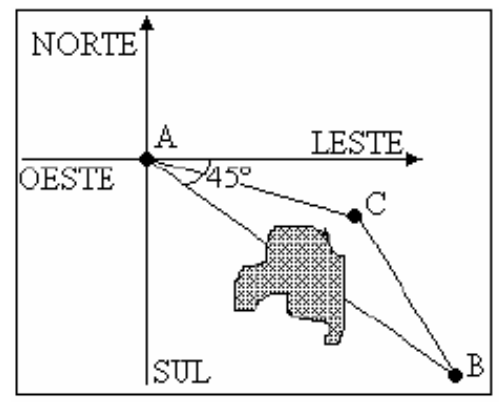
\includegraphics[width=7cm]{imgs/q21.png} % leia abaixo
\end{figure}

\begin{multicols}{3}
    \begin{enumerate}[\bf A (\quad)]
        \item 182
        \item 183
        \item 184
        \item 185
        \item n.d.a.
    \end{enumerate}
\end{multicols}

\textbf{Questão 22.} O   conjunto   dos   valores   de   $k$,   para   os   quais $f(x) = x^3 - 2x^2 + 3x - k$ tem  um  ou  três  zeros  reais  entre 1 e 2, é: 

\begin{multicols}{3}
\begin{enumerate}[\bf A (\quad)]
    \item $k < 2$
    \item $1 < k < 2$
    \item $2 > k$ ou $k > 6$
    \item $k > 7$
    \item n.d.a.
\end{enumerate}
\end{multicols}

\newpage

\textbf{Questão 23.} Seja  $c$  um  quarto  de  circunferência  $AB$  de  raio  $R$  e  centro $O$, e seja $t$ a reta tangente a $c$ em $A$. Traça-se pelo centro $O$ de $c$ uma reta que corta $c$ num ponto $M$, e corta a reta  tangente  num  ponto  $N$,  distintos  de  $A$.  Se  $k$  a  razão  entre  o  volume  gerado  pelo  setor  $OAM$  e  o  volume  gerado pelo triângulo $OAN$, ambos obtidos girando-se de $2\pi$  em torno de $AO$. O comprimento do segmento $AN$ é igual ao raio $R$ se:

\begin{figure}[h]

\centering % para centralizarmos a figura
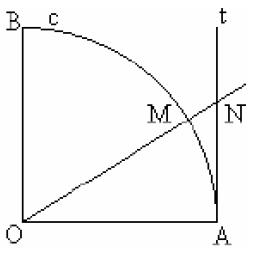
\includegraphics[width=5cm]{imgs/q23.jpg} % leia abaixo
\end{figure}

\begin{multicols}{3}
    \begin{enumerate}[\bf A (\quad)]
        \item $1 < k < 2,5$
        \item $2,5 \leq k \leq 3 $
        \item $0 < k \leq 2$
        \item $0 < k < 1,5$
        \item n.d.a.
    \end{enumerate}
\end{multicols}

\textbf{Questão 24.} Um  cone  equilátero  está  inscrito  em  uma  esfera  de  raio  4  cm.  Cortam-se  os  sólidos  (esfera  e  cone)  por  um  plano  paralelo  à  base,  de  modo  que  a  diferença  entre  as  áreas das secções seja igual à área da base do cone. O raio da secção do cone é: 

\begin{multicols}{3}
    \begin{enumerate}[\bf A (\quad)]
        \item $2\sqrt{3}$ cm
        \item $\sqrt{3}$ cm
        \item $\sqrt{3} / 3$ cm
        \item $4\sqrt{3} / 3$ cm
        \item n.d.a.
    \end{enumerate}
\end{multicols}

\textbf{Questão 25.} Seja  $a_k$  um  número  complexo,  solução  da  equação $(z + 1)^5 + z^5 = 0$,  $K  =  0,  1,  2,  3,  4$.  Podemos  afirmar  que: 


\begin{enumerate}[\bf A (\quad)]
    \item todos   os   $z_k$   ,   $K   =   0,   1, \dots,   4$   estão   sobre   uma   circunferência.
    \item todos  os  $z_k$  ,  $K  =  0,  1, \dots,  4$  estão  sobre  uma  reta  paralela ao eixo real. 
    \item todos  os  $z_k$  ,  $K  =  0,  1, \dots,  4$  estão  sobre  uma  reta  paralela ao eixo imaginário. 
    \item a equação não admite solução
    \item n.d.a.
\end{enumerate}

\end{document}